\documentclass[12pt,a4paper]{article}

% =========================================================
% PAQUETES
% =========================================================

\usepackage[utf8]{inputenc}
\usepackage[T1]{fontenc}
\usepackage[spanish]{babel}

\usepackage{geometry}
\usepackage{graphicx}
\usepackage{float}
\usepackage{xcolor}
\usepackage{listings}
\usepackage{setspace}
\usepackage{titlesec}
\usepackage{fancyhdr}
\usepackage{hyperref}
\usepackage{caption}

% =========================================================
% CONFIGURACION DE PAGINA
% =========================================================

\geometry{
    left=2.5cm,
    right=2.5cm,
    top=2.5cm,
    bottom=2.5cm
}

% formato de parrafos
\setlength{\parindent}{0pt}
\setlength{\parskip}{0.6em}

\setstretch{1.2}

% corrige el warning de fancyhdr
\setlength{\headheight}{15pt}

% carpeta donde estan las capturas
\graphicspath{{imagenes/}}

% =========================================================
% COLORES
% =========================================================

\definecolor{azultitulo}{RGB}{35,85,140}
\definecolor{grisclaro}{RGB}{245,245,245}
\definecolor{grislinea}{RGB}{180,180,180}

% =========================================================
% TITULOS
% =========================================================

\titleformat{\section}
{\Large\bfseries\color{azultitulo}}
{\thesection.}
{0.5em}
{}

\titleformat{\subsection}
{\large\bfseries}
{\thesubsection}
{0.5em}
{}

% =========================================================
% CODIGO EN C
% =========================================================

\lstdefinestyle{codigoC}{
    language=C,
    basicstyle=\ttfamily\small,
    breaklines=true,
    frame=single,
    rulecolor=\color{grislinea},
    backgroundcolor=\color{grisclaro},
    numbers=left,
    numberstyle=\tiny,
    numbersep=8pt,
    showstringspaces=false,
    tabsize=4,
    columns=fullflexible
}

% =========================================================
% ENCABEZADO Y PIE DE PAGINA
% =========================================================

\pagestyle{fancy}
\fancyhf{}

\fancyhead[L]{Microcontroladores}
\fancyhead[R]{Trabajo Colaborativo 2}

\fancyfoot[C]{\thepage}

% =========================================================
% DOCUMENTO
% =========================================================

\begin{document}

% =========================================================
% PORTADA
% =========================================================

\pagenumbering{gobble}

\begin{titlepage}

    \centering

    {\Large Universidad Andrés Bello\par}

    \vspace{1.5cm}

    {\Large Ingeniería en Automatización y Robótica\par}

    \vspace{2cm}

    {\Huge\textbf{Trabajo Colaborativo N°2}\par}

    \vspace{0.5cm}

    {\LARGE Manejo de Entradas y Salidas Digitales\par}

    \vspace{2cm}

    {\large Asignatura: Microcontroladores\par}

    \vspace{0.4cm}

    {\large Código: AAUT103\par}

    \vfill

    {\large\textbf{Integrantes}\par}

    \vspace{0.5cm}

    {\large Alex Díaz\par}

    \vspace{0.2cm}

    {\large María José Córdova\par}

    \vfill

    {\large 2026\par}

\end{titlepage}

% =========================================================
% INDICE
% =========================================================

\tableofcontents

\clearpage

\pagenumbering{arabic}

% =========================================================
% INTRODUCCION
% =========================================================

\section{Introducción}

En este trabajo colaborativo se desarrollaron distintas actividades de programación y simulación utilizando el microcontrolador PIC16F877A. Para esto se utilizó MPLAB X junto al compilador XC8 para generar los archivos \texttt{.hex}, y SimulIDE para comprobar el funcionamiento de los circuitos.

Las actividades permitieron trabajar progresivamente con salidas digitales, entradas mediante pulsadores y el control de varios LED, hasta llegar a la implementación de un sistema de dos semáforos controlados mediante el microcontrolador.

Durante el desarrollo se trabajó con los registros de configuración de entradas y salidas, principalmente TRIS y PORT, además de la configuración necesaria para utilizar pines del puerto A como entradas digitales.

% =========================================================
% ACTIVIDAD 1
% =========================================================

\section{Actividad 1: LED parpadeante}

En esta primera actividad se compiló y simuló un programa básico para controlar un LED conectado al pin RB0 del microcontrolador PIC16F877A.

El programa enciende el LED durante 500 milisegundos y posteriormente lo apaga durante otros 500 milisegundos, repitiendo este comportamiento de forma continua.

El código utilizado corresponde al programa entregado en la guía del trabajo colaborativo.

\subsection{Programa utilizado}

\begin{lstlisting}[style=codigoC]
/*
 * descripcion: programa basico para encender un led conectado
 * al pin rb0 del pic16f877a
 */

// configuracion del pic
#pragma config FOSC = XT
#pragma config WDTE = OFF
#pragma config PWRTE = ON
#pragma config BOREN = ON
#pragma config LVP = OFF
#pragma config CPD = OFF
#pragma config WRT = OFF
#pragma config CP = OFF

// libreria principal para usar el pic con xc8
#include <xc.h>

// frecuencia del cristal de 4 mhz
#define _XTAL_FREQ 4000000

// nombre que usaremos para el pin rb0
#define LED RB0

void main(void)
{
    // configura todo el puerto b como salida
    TRISB = 0x00;

    // deja todas las salidas del puerto b apagadas al iniciar
    PORTB = 0x00;

    // el programa se repite para siempre
    while (1)
    {
        // enciende el led
        LED = 1;

        // espera 500 milisegundos
        __delay_ms(500);

        // apaga el led
        LED = 0;

        // espera otros 500 milisegundos
        __delay_ms(500);
    }

    return;
}
\end{lstlisting}

\subsection{Resultado de la simulación}

En la siguiente captura se puede observar la compilación correcta del programa en MPLAB X y la ejecución del circuito en SimulIDE.

\begin{figure}[H]
    \centering

    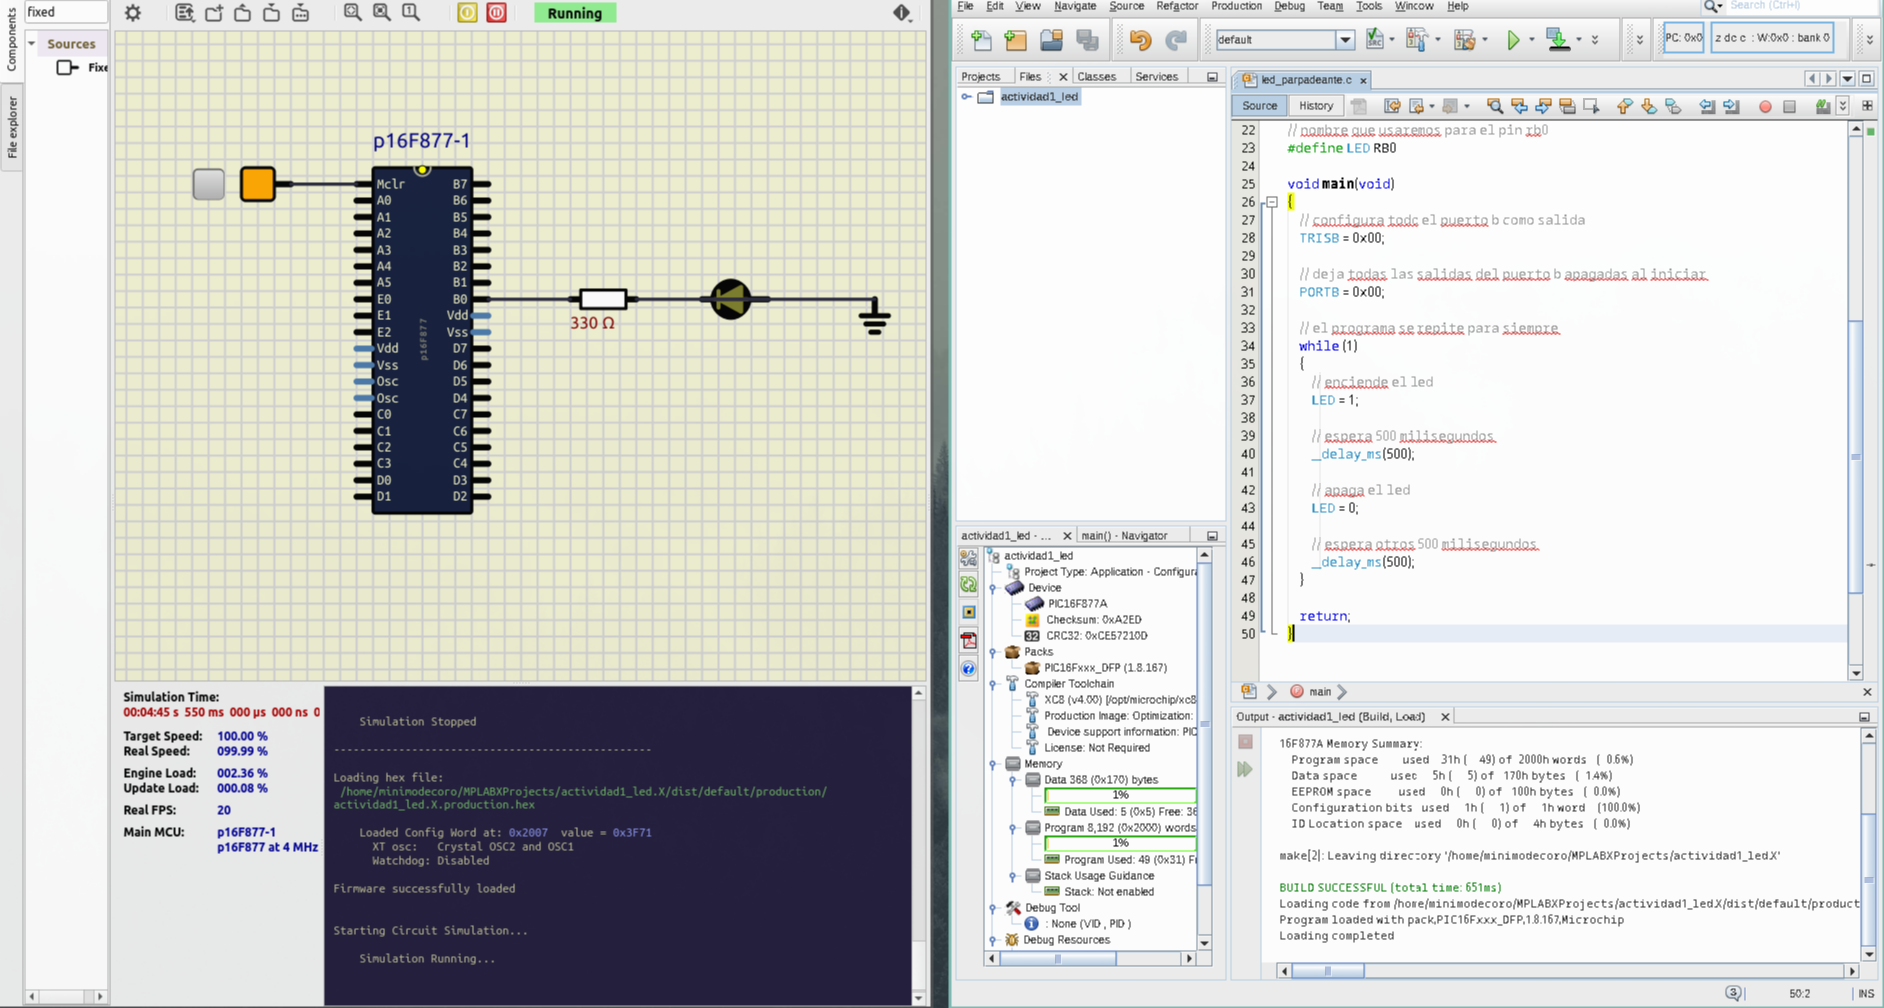
\includegraphics[
        width=0.95\textwidth,
        height=0.72\textheight,
        keepaspectratio
    ]{actividad1_simulide.png}

    \caption{Compilación en MPLAB X y simulación del LED parpadeante en SimulIDE.}
\end{figure}

\clearpage

% =========================================================
% ACTIVIDAD 2
% =========================================================

\section{Actividad 2: Control de LED mediante pulsador}

En esta actividad se utilizó un pulsador conectado al pin RA0 como entrada digital y un LED conectado al pin RB0 como salida.

El pulsador fue configurado mediante una resistencia pull-up, por lo que al encontrarse sin presionar la entrada permanece en estado lógico alto, mientras que al presionarlo la entrada cambia a estado lógico bajo.

El programa detecta este cambio y enciende el LED mientras el pulsador se encuentra presionado.

\subsection{Programa realizado}

\begin{lstlisting}[style=codigoC]
/*
 * descripcion: enciende un led cuando se presiona un pulsador
 * y lo apaga cuando se suelta
 */

// configuracion del pic
#pragma config FOSC = XT
#pragma config WDTE = OFF
#pragma config PWRTE = ON
#pragma config BOREN = ON
#pragma config LVP = OFF
#pragma config CPD = OFF
#pragma config WRT = OFF
#pragma config CP = OFF

// libreria principal para usar el pic con xc8
#include <xc.h>

// frecuencia del cristal
#define _XTAL_FREQ 4000000

// led conectado a rb0
#define LED RB0

// pulsador conectado a ra0
#define PULSADOR RA0

void main(void)
{
    // convierte los pines analogicos del puerto a en digitales
    ADCON1 = 0x06;

    // rb0 sera salida para el led
    TRISBbits.TRISB0 = 0;

    // ra0 sera entrada para el pulsador
    TRISAbits.TRISA0 = 1;

    // parte con el led apagado
    PORTB = 0x00;

    // el programa se repite para siempre
    while(1)
    {
        // con pull-up, al presionar el boton ra0 pasa a 0
        if(PULSADOR == 0)
        {
            // boton presionado
            LED = 1;
        }
        else
        {
            // boton suelto
            LED = 0;
        }
    }

    return;
}
\end{lstlisting}

\subsection{Resultado de la simulación}

La primera captura muestra el LED apagado cuando el pulsador se encuentra sin presionar.

\begin{figure}[H]
    \centering

    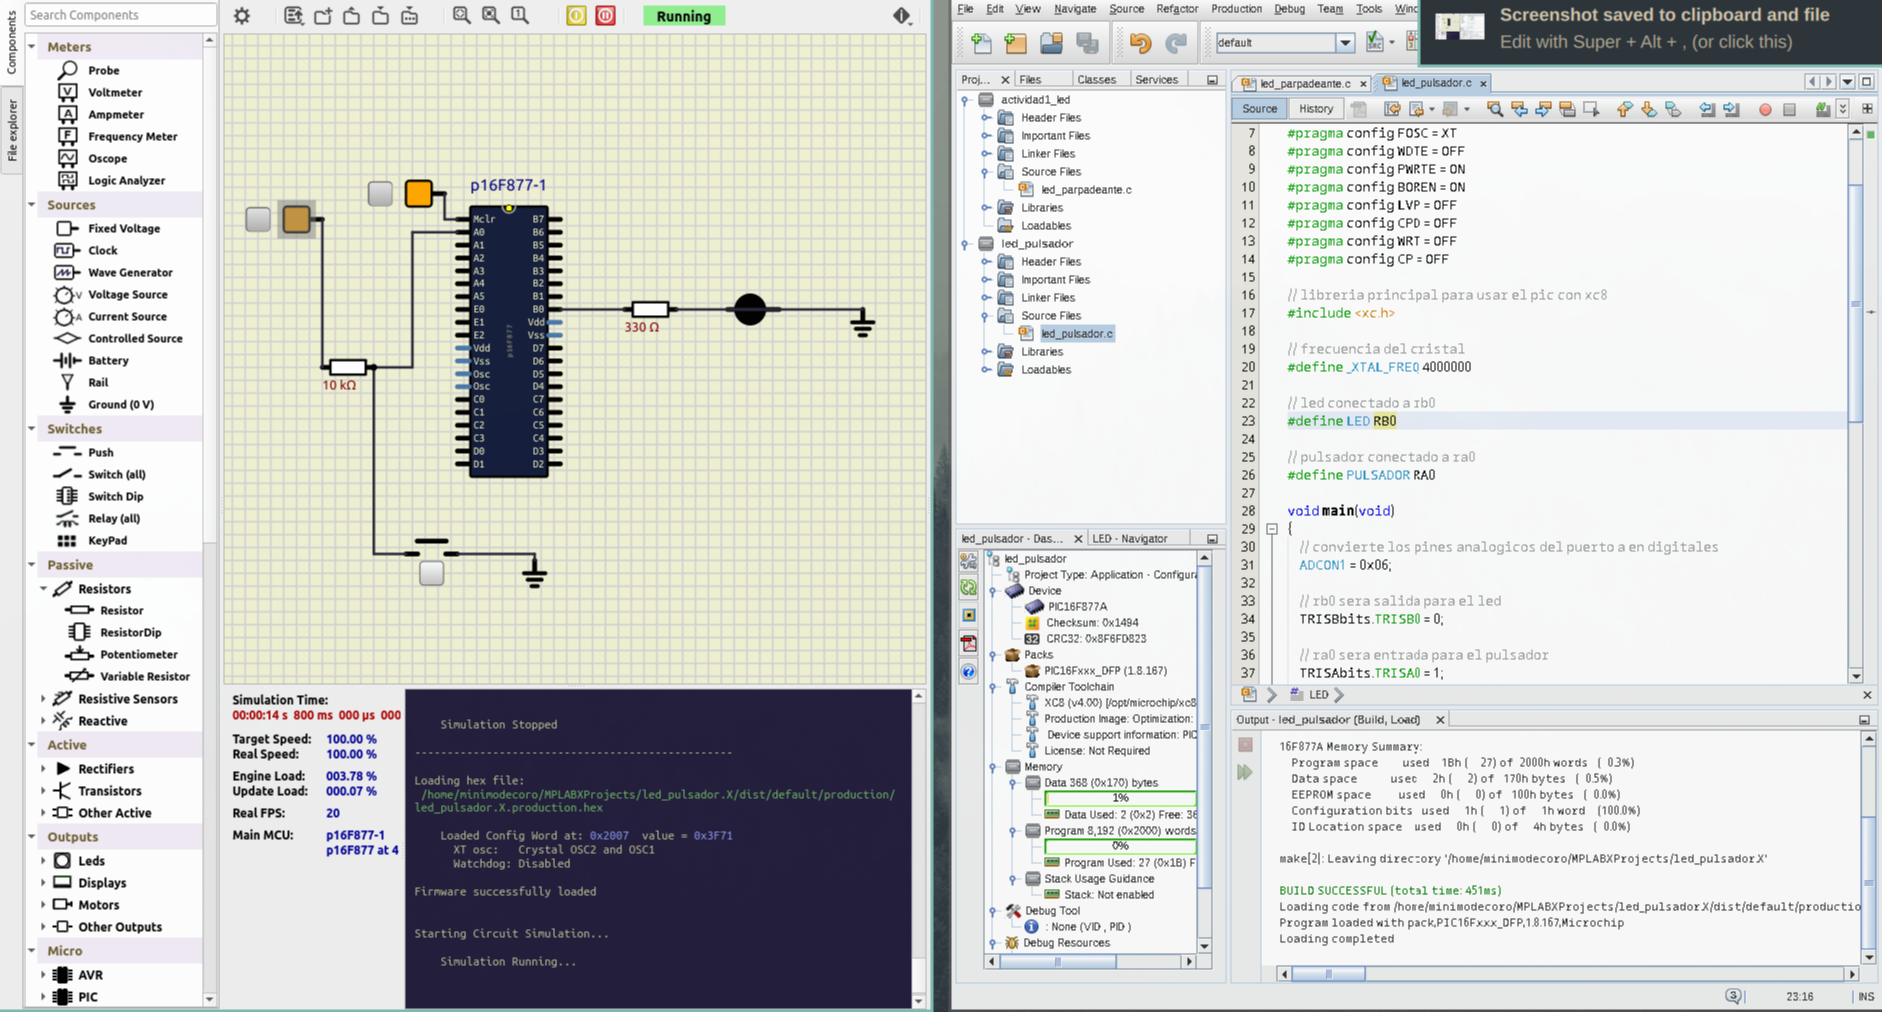
\includegraphics[
        width=0.88\textwidth,
        height=0.7\textheight,
        keepaspectratio
    ]{actividad2_apagado.png}

    \caption{Actividad 2 con el LED apagado.}
\end{figure}

La segunda captura muestra el LED encendido al accionar el pulsador.

\begin{figure}[H]
    \centering

    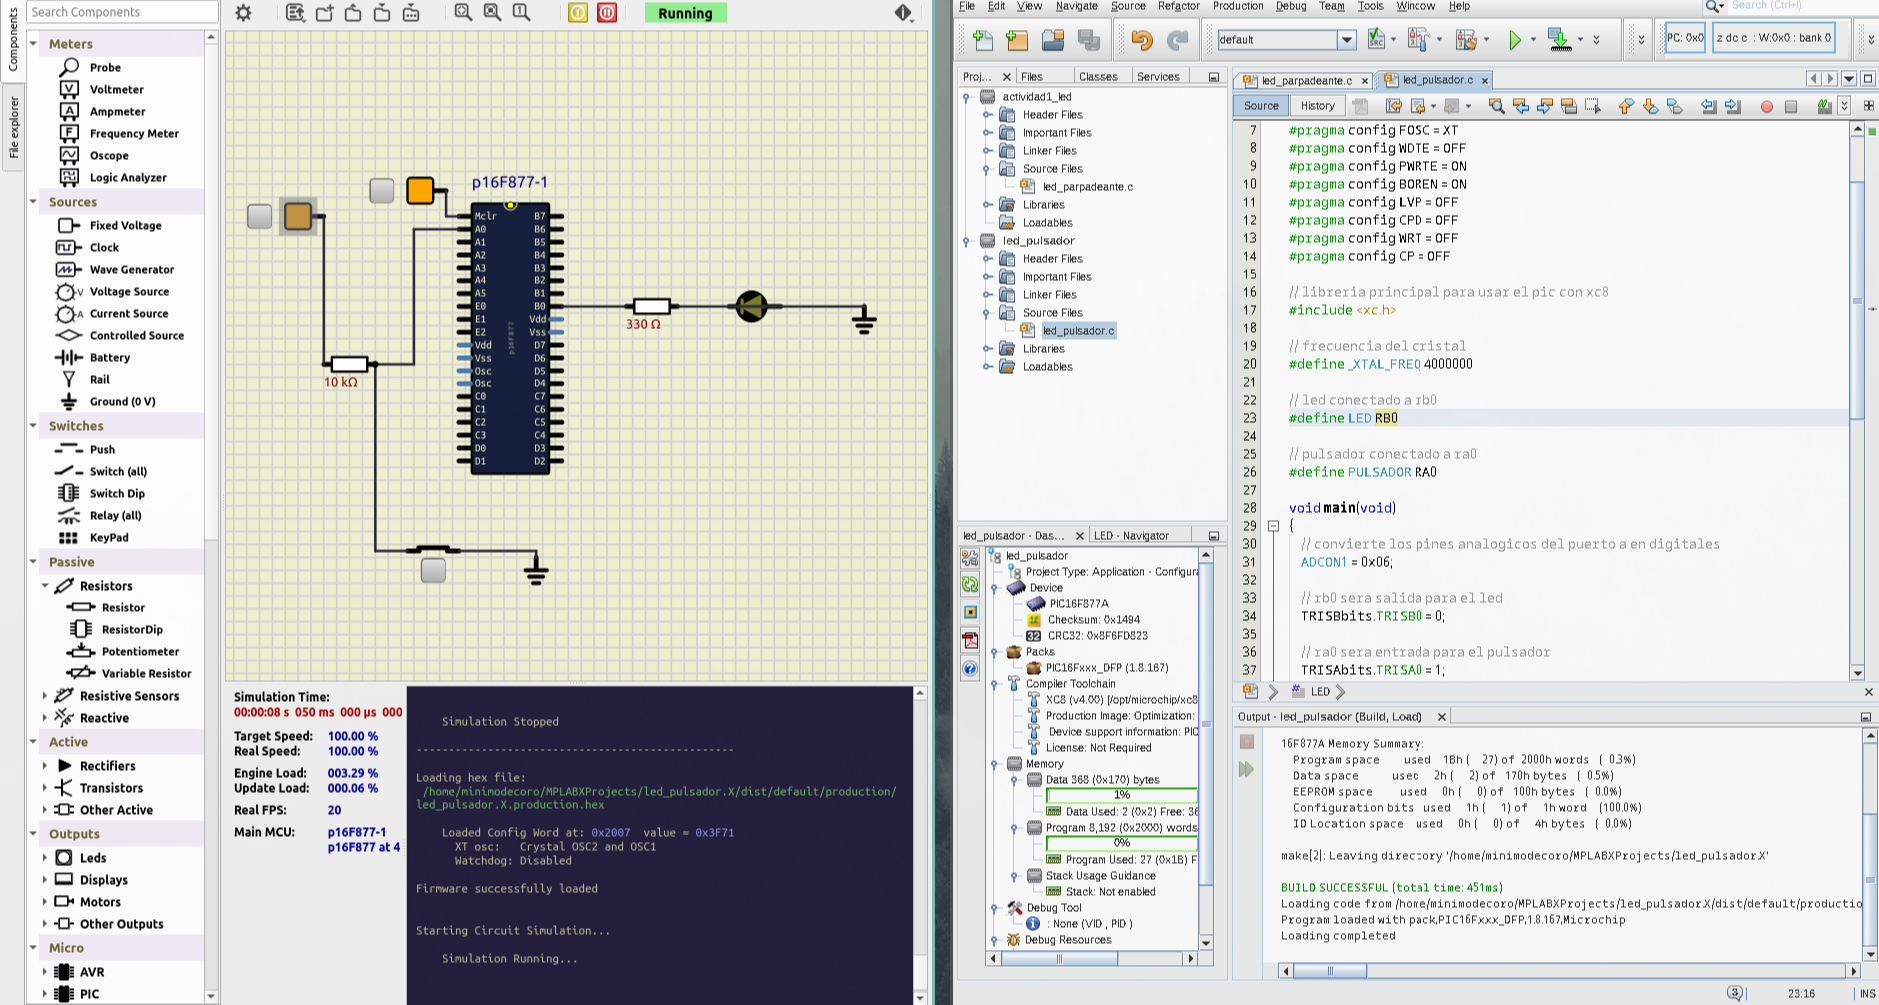
\includegraphics[
        width=0.88\textwidth,
        height=0.7\textheight,
        keepaspectratio
    ]{actividad2_encendido.png}

    \caption{Actividad 2 con el LED encendido.}
\end{figure}

\clearpage

% =========================================================
% ACTIVIDAD 3
% =========================================================

\section{Actividad 3: Control alternado de dos LED}

En esta actividad se utilizaron dos LED conectados a los pines RB0 y RB1.

El pulsador conectado a RA0 permite cambiar entre dos estados. En uno de ellos se encuentra encendido el primer LED y apagado el segundo, mientras que al presionar el pulsador estos estados se invierten.

\subsection{Programa realizado}

\begin{lstlisting}[style=codigoC]
/*
 * descripcion: controla dos leds de forma alternada
 * mediante un pulsador
 */

// configuracion del pic
#pragma config FOSC = XT
#pragma config WDTE = OFF
#pragma config PWRTE = ON
#pragma config BOREN = ON
#pragma config LVP = OFF
#pragma config CPD = OFF
#pragma config WRT = OFF
#pragma config CP = OFF

// libreria principal para usar el pic con xc8
#include <xc.h>

// frecuencia del cristal
#define _XTAL_FREQ 4000000

// leds conectados al puerto b
#define LED1 RB0
#define LED2 RB1

// pulsador conectado a ra0
#define PULSADOR RA0

void main(void)
{
    // convierte los pines analogicos del puerto a en digitales
    ADCON1 = 0x06;

    // rb0 sera salida para el led 1
    TRISBbits.TRISB0 = 0;

    // rb1 sera salida para el led 2
    TRISBbits.TRISB1 = 0;

    // ra0 sera entrada para el pulsador
    TRISAbits.TRISA0 = 1;

    // deja el puerto b apagado al iniciar
    PORTB = 0x00;

    // el programa se repite para siempre
    while(1)
    {
        // si el boton esta presionado
        if(PULSADOR == 0)
        {
            // apaga el led 1
            LED1 = 0;

            // enciende el led 2
            LED2 = 1;
        }
        else
        {
            // enciende el led 1
            LED1 = 1;

            // apaga el led 2
            LED2 = 0;
        }
    }

    return;
}
\end{lstlisting}

\subsection{Resultado de la simulación}

\begin{figure}[H]
    \centering

    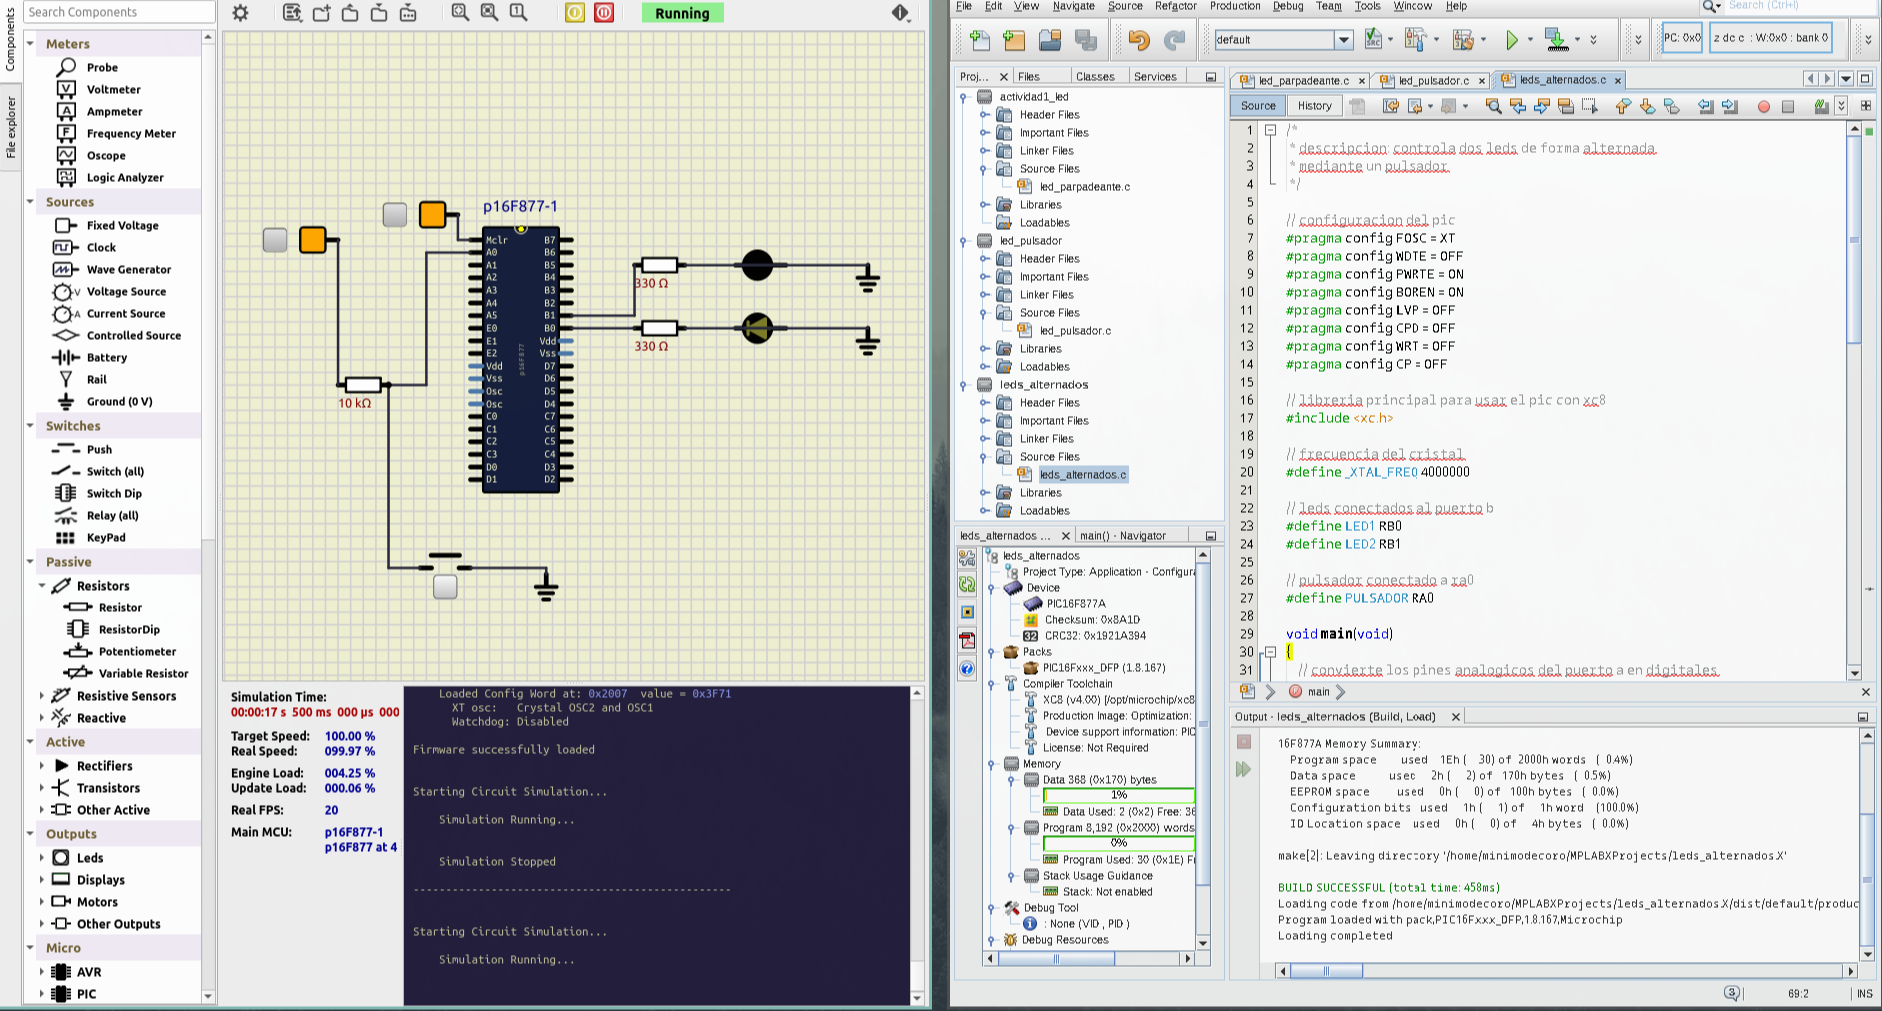
\includegraphics[
        width=0.88\textwidth,
        height=0.7\textheight,
        keepaspectratio
    ]{actividad3_led1.png}

    \caption{Primer estado de la actividad 3: LED 1 encendido y LED 2 apagado.}
\end{figure}

\begin{figure}[H]
    \centering

    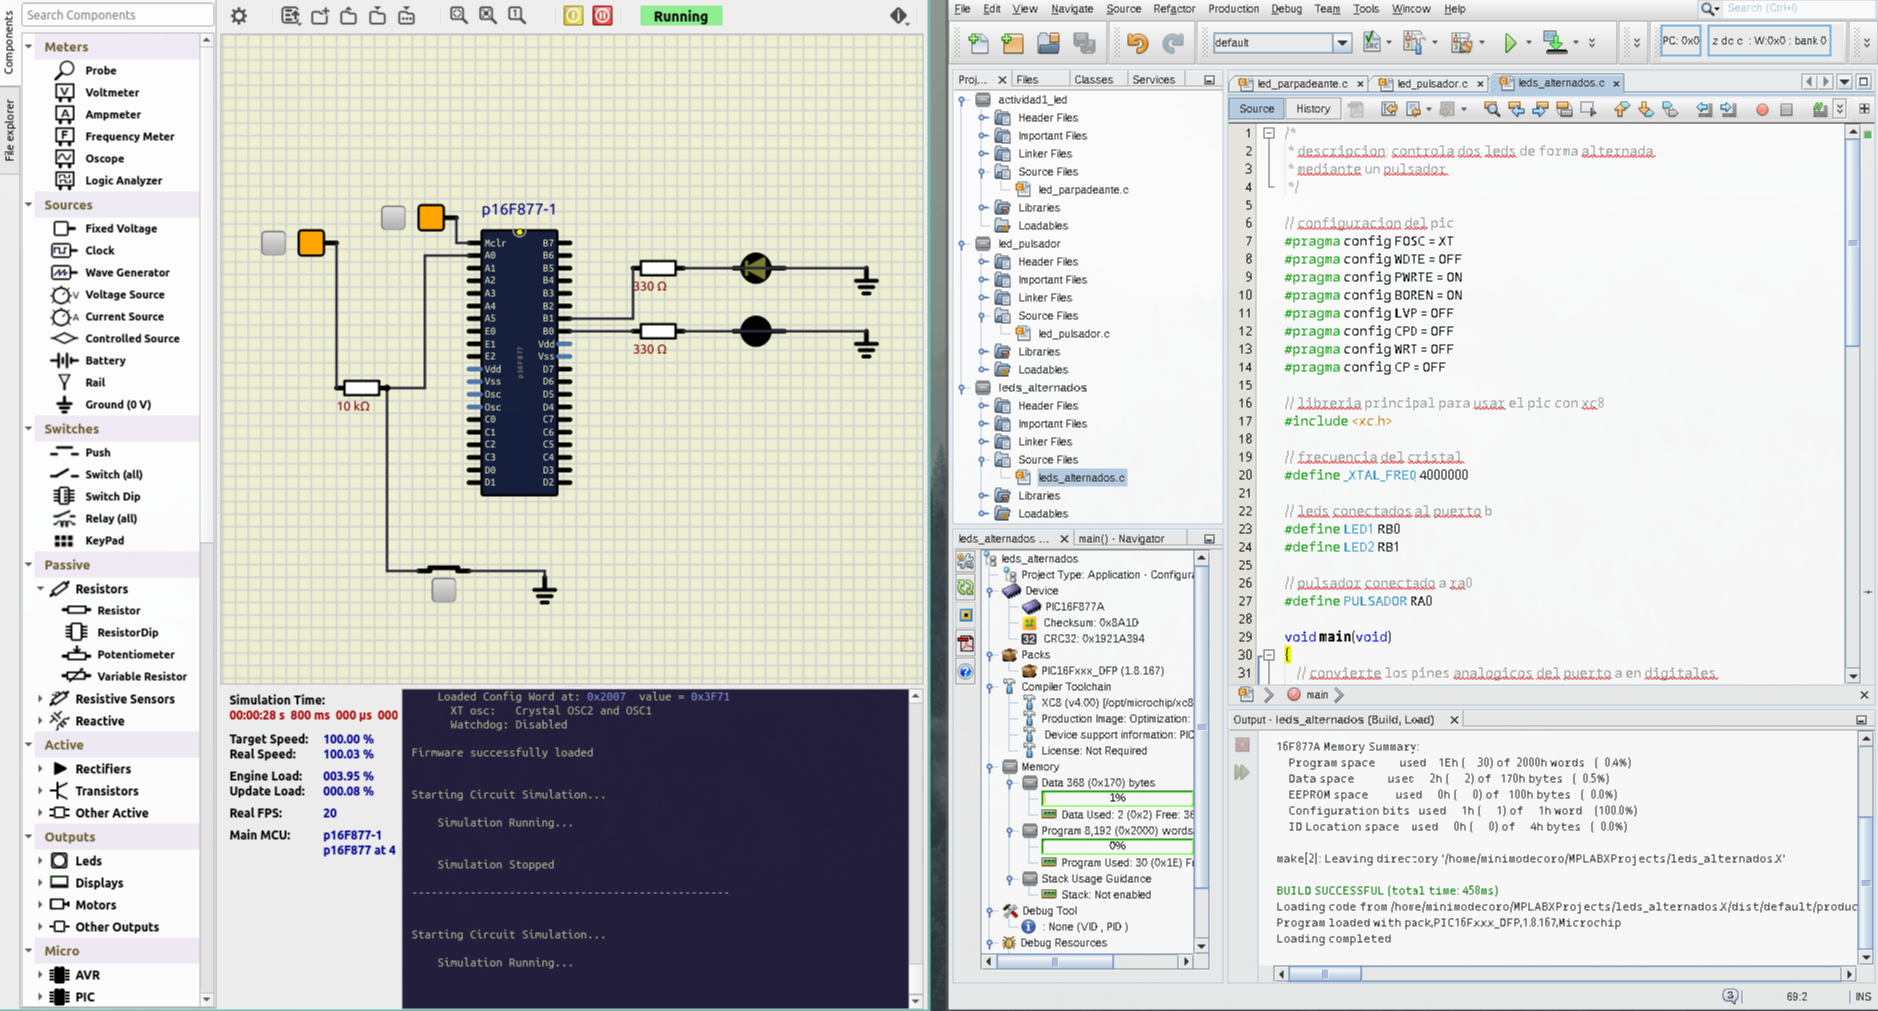
\includegraphics[
        width=0.88\textwidth,
        height=0.7\textheight,
        keepaspectratio
    ]{actividad3_led2.png}

    \caption{Segundo estado de la actividad 3: LED 1 apagado y LED 2 encendido.}
\end{figure}

\clearpage

% =========================================================
% ACTIVIDAD 4
% =========================================================

\section{Actividad 4: Control de un LED mediante dos pulsadores}

Para esta actividad se utilizaron dos pulsadores independientes.

El primer pulsador se encuentra conectado al pin RA0 y permite encender el LED. El segundo se encuentra conectado al pin RA1 y permite apagarlo.

Una vez encendido, el LED mantiene su estado hasta que se acciona el pulsador de apagado.

\subsection{Programa realizado}

\begin{lstlisting}[style=codigoC]
/*
 * descripcion: enciende un led con un pulsador
 * y lo apaga con otro pulsador
 */

// configuracion del pic
#pragma config FOSC = XT
#pragma config WDTE = OFF
#pragma config PWRTE = ON
#pragma config BOREN = ON
#pragma config LVP = OFF
#pragma config CPD = OFF
#pragma config WRT = OFF
#pragma config CP = OFF

// libreria principal para usar el pic con xc8
#include <xc.h>

// frecuencia del cristal
#define _XTAL_FREQ 4000000

// led conectado a rb0
#define LED RB0

// pulsador de encendido conectado a ra0
#define BOTON_ON RA0

// pulsador de apagado conectado a ra1
#define BOTON_OFF RA1

void main(void)
{
    // convierte los pines analogicos del puerto a en digitales
    ADCON1 = 0x06;

    // rb0 sera salida para el led
    TRISBbits.TRISB0 = 0;

    // ra0 sera entrada para el boton de encendido
    TRISAbits.TRISA0 = 1;

    // ra1 sera entrada para el boton de apagado
    TRISAbits.TRISA1 = 1;

    // el led parte apagado
    LED = 0;

    // el programa se repite para siempre
    while(1)
    {
        // si se presiona el boton de encendido
        if(BOTON_ON == 0)
        {
            LED = 1;
        }

        // si se presiona el boton de apagado
        if(BOTON_OFF == 0)
        {
            LED = 0;
        }
    }

    return;
}
\end{lstlisting}

\subsection{Resultado de la simulación}

\begin{figure}[H]
    \centering

    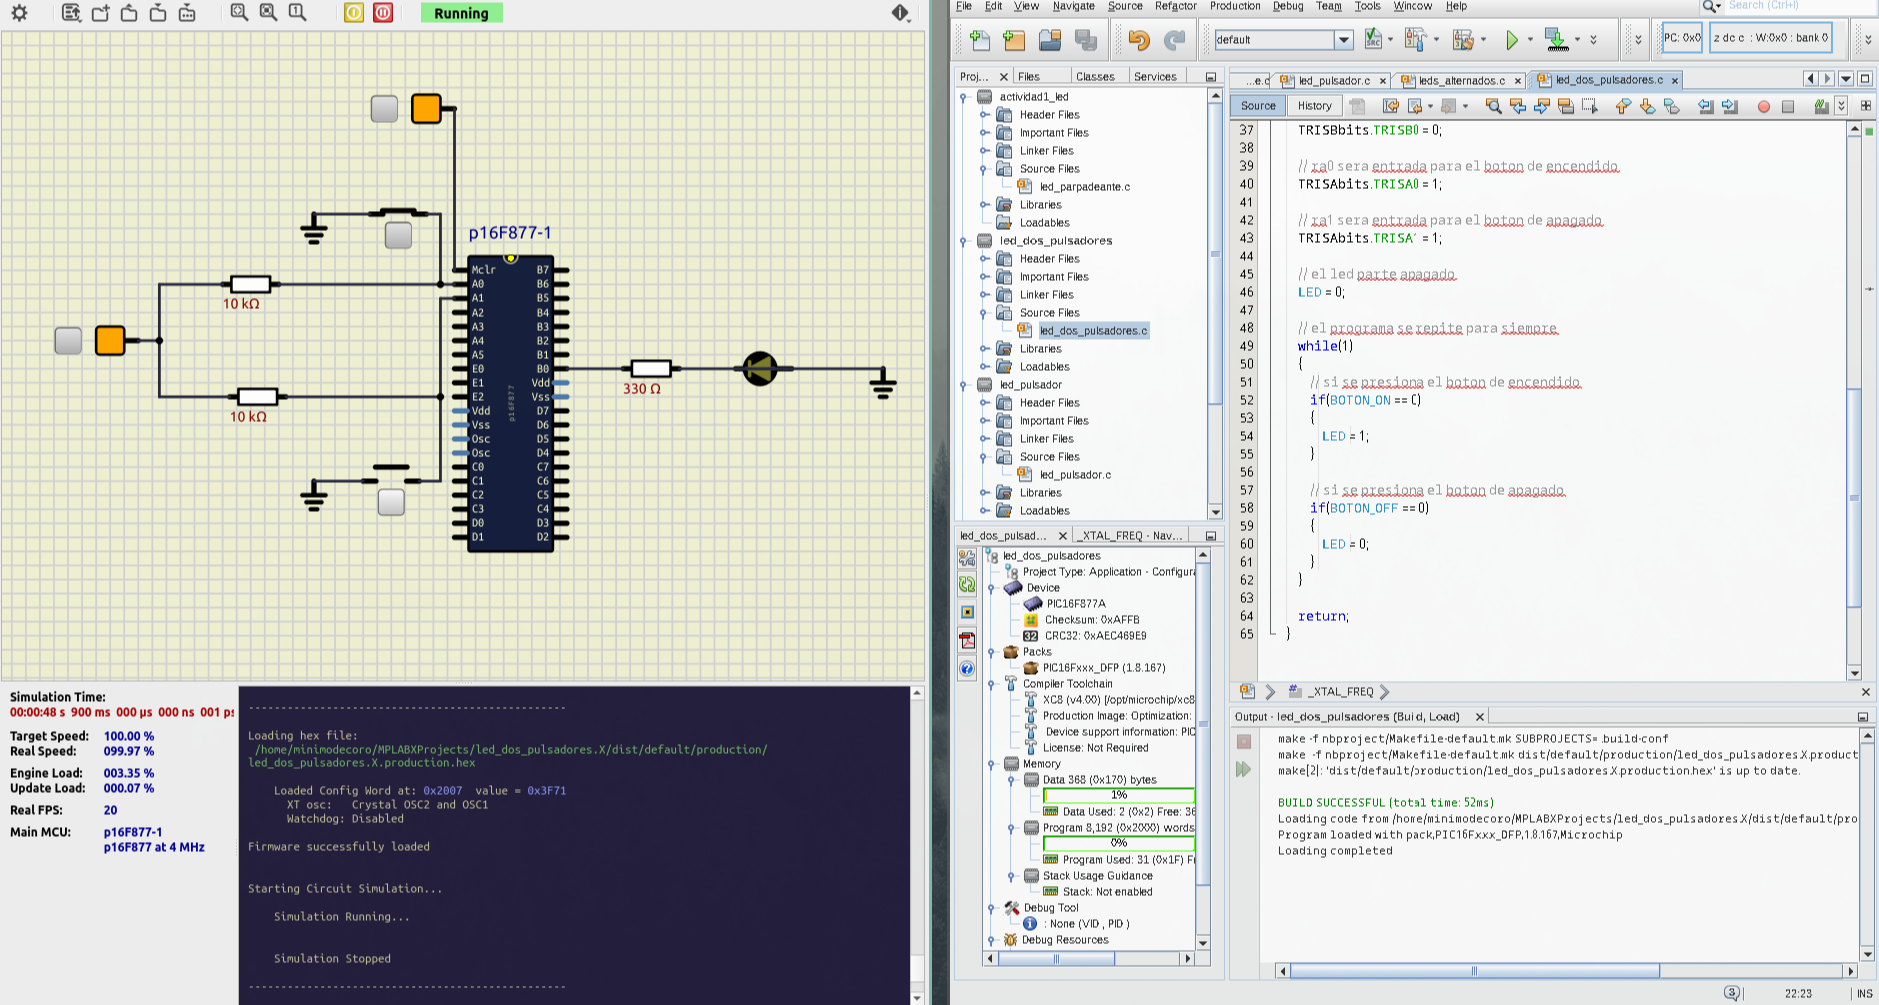
\includegraphics[
        width=0.88\textwidth,
        height=0.7\textheight,
        keepaspectratio
    ]{actividad4_encendido.png}

    \caption{LED encendido mediante el pulsador conectado a RA0.}
\end{figure}

\begin{figure}[H]
    \centering

    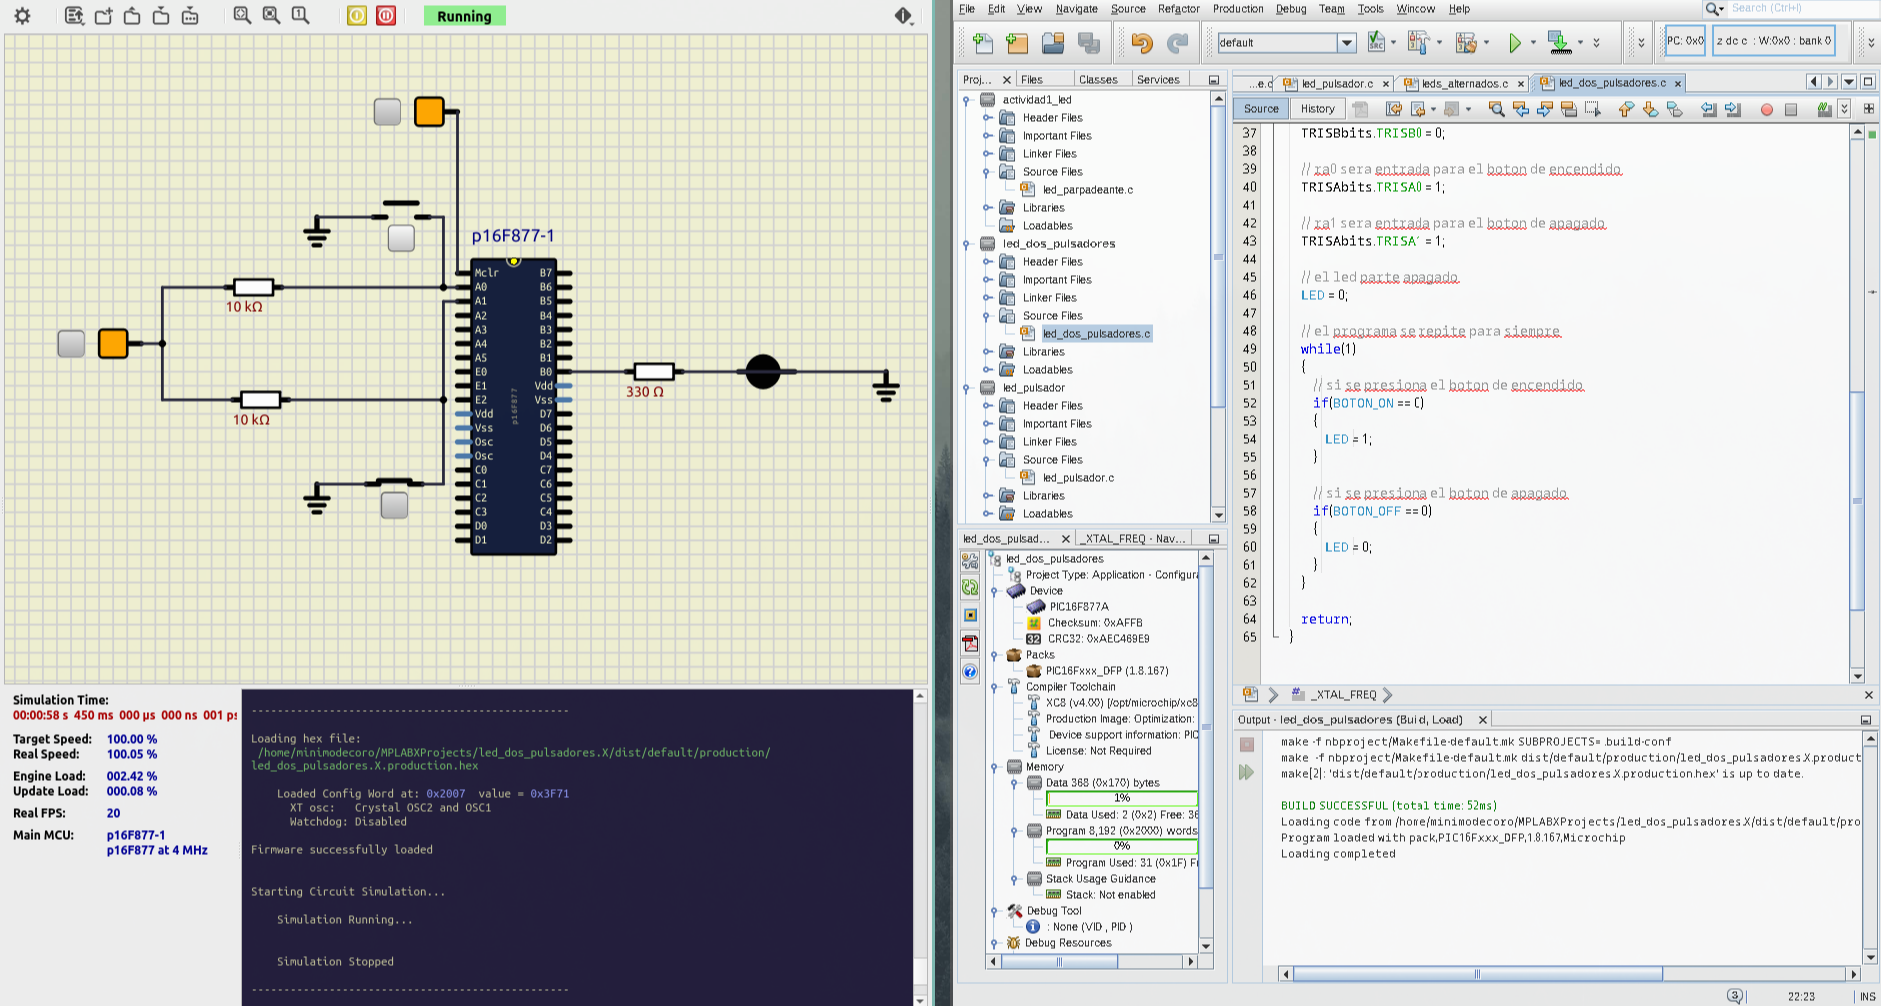
\includegraphics[
        width=0.88\textwidth,
        height=0.7\textheight,
        keepaspectratio
    ]{actividad4_apagado.png}

    \caption{LED apagado mediante el pulsador conectado a RA1.}
\end{figure}

\clearpage

% =========================================================
% ACTIVIDAD 5
% =========================================================

\section{Actividad 5: Semáforo con un PIC}

En la última actividad se implementó el control de dos semáforos utilizando seis LED.

El primer semáforo utiliza los pines RB0, RB1 y RB2 para sus luces verde, amarilla y roja respectivamente.

El segundo semáforo utiliza los pines RB3, RB4 y RB5.

Además, se utiliza una entrada en RA0 para activar la secuencia mediante un interruptor.

El programa ejecuta cuatro fases de un segundo cada una y repite el ciclo mientras el interruptor se encuentra activado.

\subsection{Programa realizado}

\begin{lstlisting}[style=codigoC]
/*
 * descripcion: controla dos semaforos con seis leds
 * la secuencia funciona mientras el interruptor esta activado
 */

// configuracion del pic
#pragma config FOSC = XT
#pragma config WDTE = OFF
#pragma config PWRTE = ON
#pragma config BOREN = ON
#pragma config LVP = OFF
#pragma config CPD = OFF
#pragma config WRT = OFF
#pragma config CP = OFF

// libreria principal para usar el pic con xc8
#include <xc.h>

// frecuencia del cristal
#define _XTAL_FREQ 4000000

// semaforo 1
#define VERDE1 RB0
#define AMARILLO1 RB1
#define ROJO1 RB2

// semaforo 2
#define VERDE2 RB3
#define AMARILLO2 RB4
#define ROJO2 RB5

// interruptor conectado a ra0
#define INTERRUPTOR RA0

void main(void)
{
    // convierte los pines analogicos del puerto a en digitales
    ADCON1 = 0x06;

    // rb0 a rb5 seran salidas
    TRISBbits.TRISB0 = 0;
    TRISBbits.TRISB1 = 0;
    TRISBbits.TRISB2 = 0;
    TRISBbits.TRISB3 = 0;
    TRISBbits.TRISB4 = 0;
    TRISBbits.TRISB5 = 0;

    // ra0 sera entrada para el interruptor
    TRISAbits.TRISA0 = 1;

    // todos los leds parten apagados
    PORTB = 0x00;

    while(1)
    {
        // si el interruptor esta activado
        if(INTERRUPTOR == 0)
        {
            // fase 1
            // semaforo 1 verde
            // semaforo 2 rojo

            VERDE1 = 1;
            AMARILLO1 = 0;
            ROJO1 = 0;

            VERDE2 = 0;
            AMARILLO2 = 0;
            ROJO2 = 1;

            __delay_ms(1000);

            // fase 2
            // semaforo 1 amarillo
            // semaforo 2 rojo

            VERDE1 = 0;
            AMARILLO1 = 1;
            ROJO1 = 0;

            VERDE2 = 0;
            AMARILLO2 = 0;
            ROJO2 = 1;

            __delay_ms(1000);

            // fase 3
            // semaforo 1 rojo
            // semaforo 2 verde

            VERDE1 = 0;
            AMARILLO1 = 0;
            ROJO1 = 1;

            VERDE2 = 1;
            AMARILLO2 = 0;
            ROJO2 = 0;

            __delay_ms(1000);

            // fase 4
            // semaforo 1 rojo
            // semaforo 2 amarillo

            VERDE1 = 0;
            AMARILLO1 = 0;
            ROJO1 = 1;

            VERDE2 = 0;
            AMARILLO2 = 1;
            ROJO2 = 0;

            __delay_ms(1000);
        }
        else
        {
            // si el interruptor esta apagado
            // se apagan todos los leds
            PORTB = 0x00;
        }
    }

    return;
}
\end{lstlisting}

\subsection{Fase 1}

En la primera fase, el semáforo 1 mantiene encendida la luz verde, mientras que el semáforo 2 mantiene encendida la luz roja.

\begin{figure}[H]
    \centering

    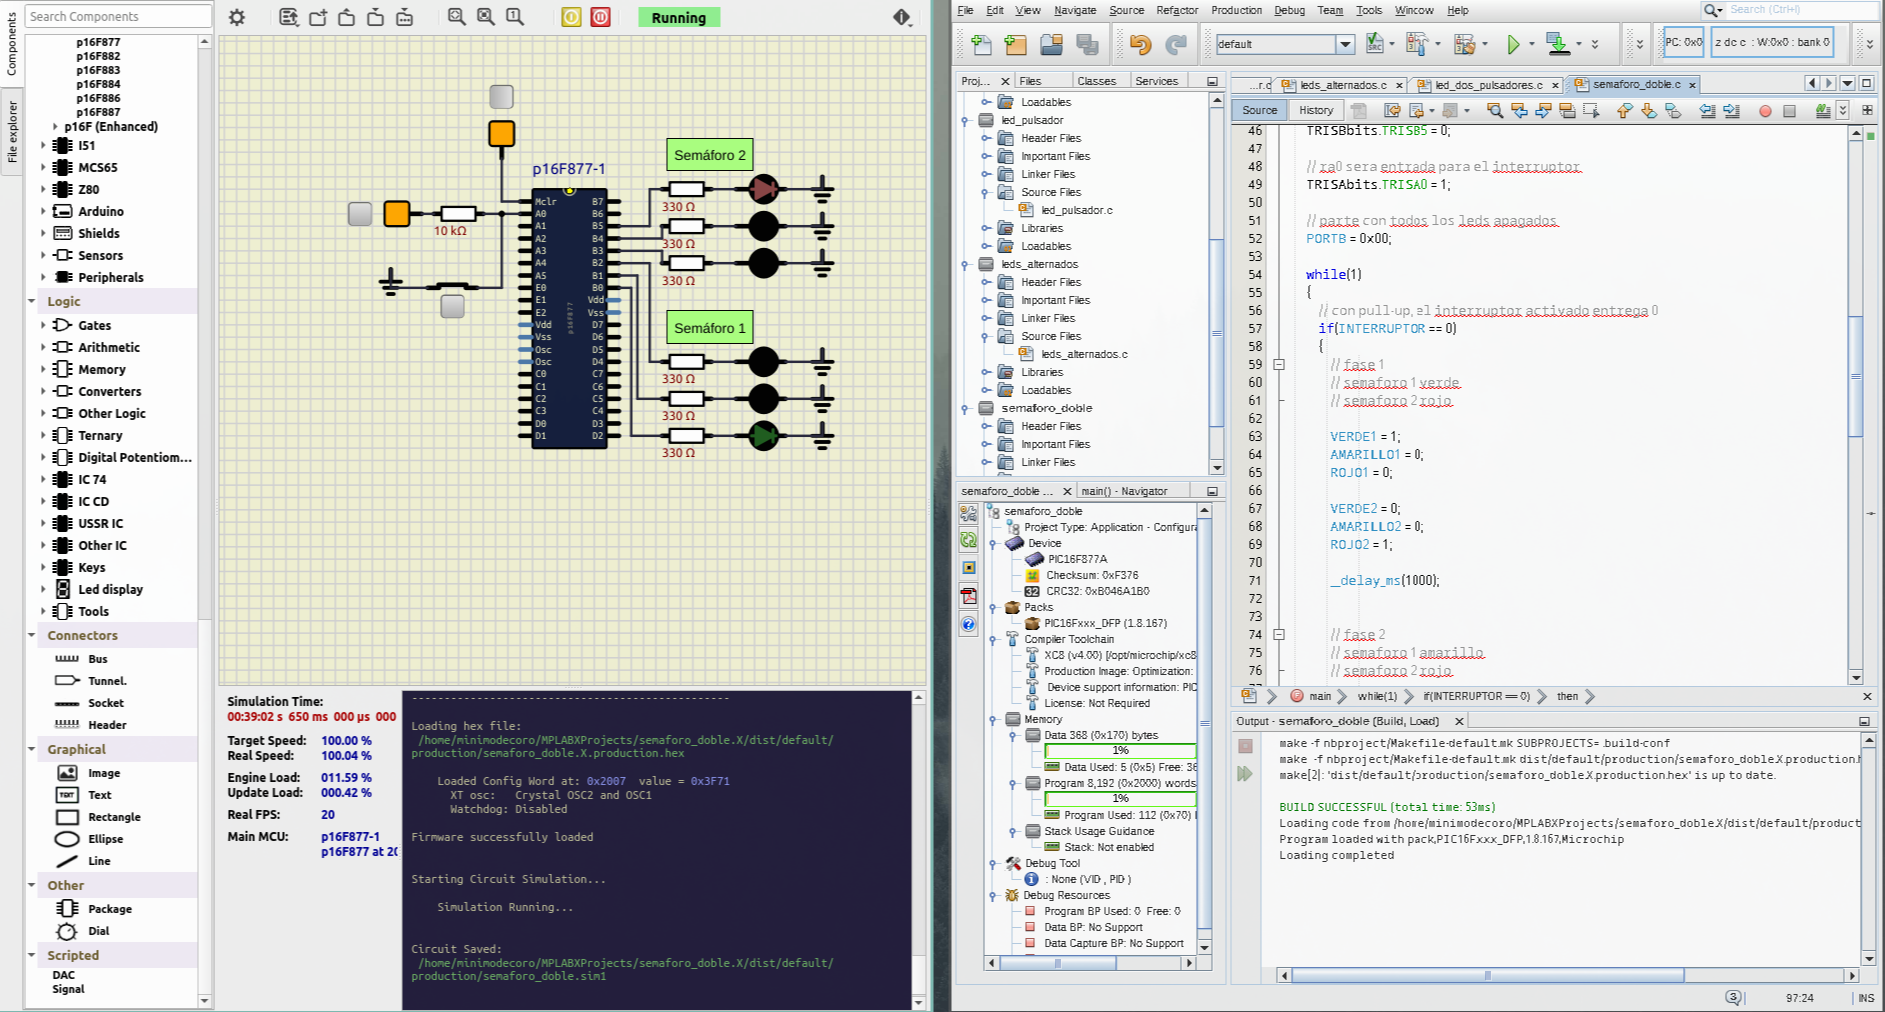
\includegraphics[
        width=0.9\textwidth,
        height=0.7\textheight,
        keepaspectratio
    ]{actividad5_fase1.png}

    \caption{Fase 1: semáforo 1 en verde y semáforo 2 en rojo.}
\end{figure}

\subsection{Fase 2}

En la segunda fase, el semáforo 1 cambia a amarillo, mientras que el semáforo 2 continúa en rojo.

\begin{figure}[H]
    \centering

    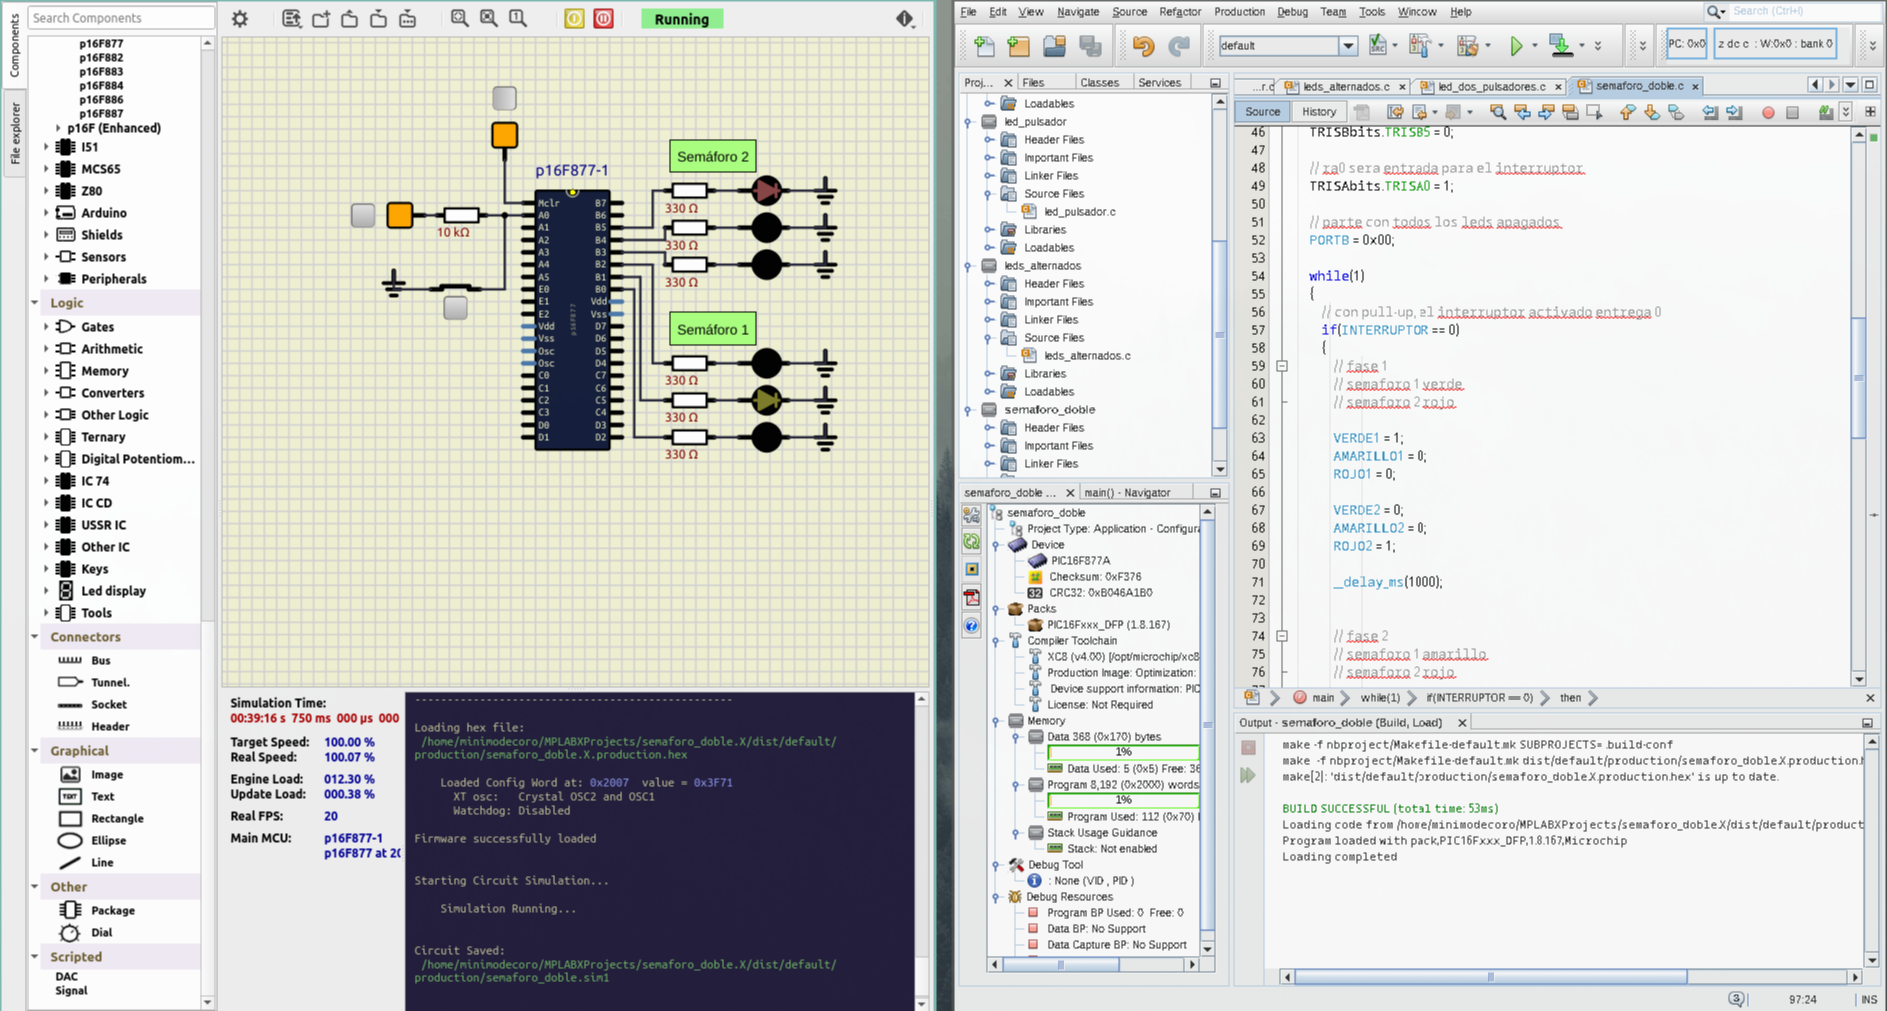
\includegraphics[
        width=0.9\textwidth,
        height=0.7\textheight,
        keepaspectratio
    ]{actividad5_fase2.png}

    \caption{Fase 2: semáforo 1 en amarillo y semáforo 2 en rojo.}
\end{figure}

\subsection{Fase 3}

En la tercera fase, el semáforo 1 mantiene encendida la luz roja y el semáforo 2 cambia a verde.

\begin{figure}[H]
    \centering

    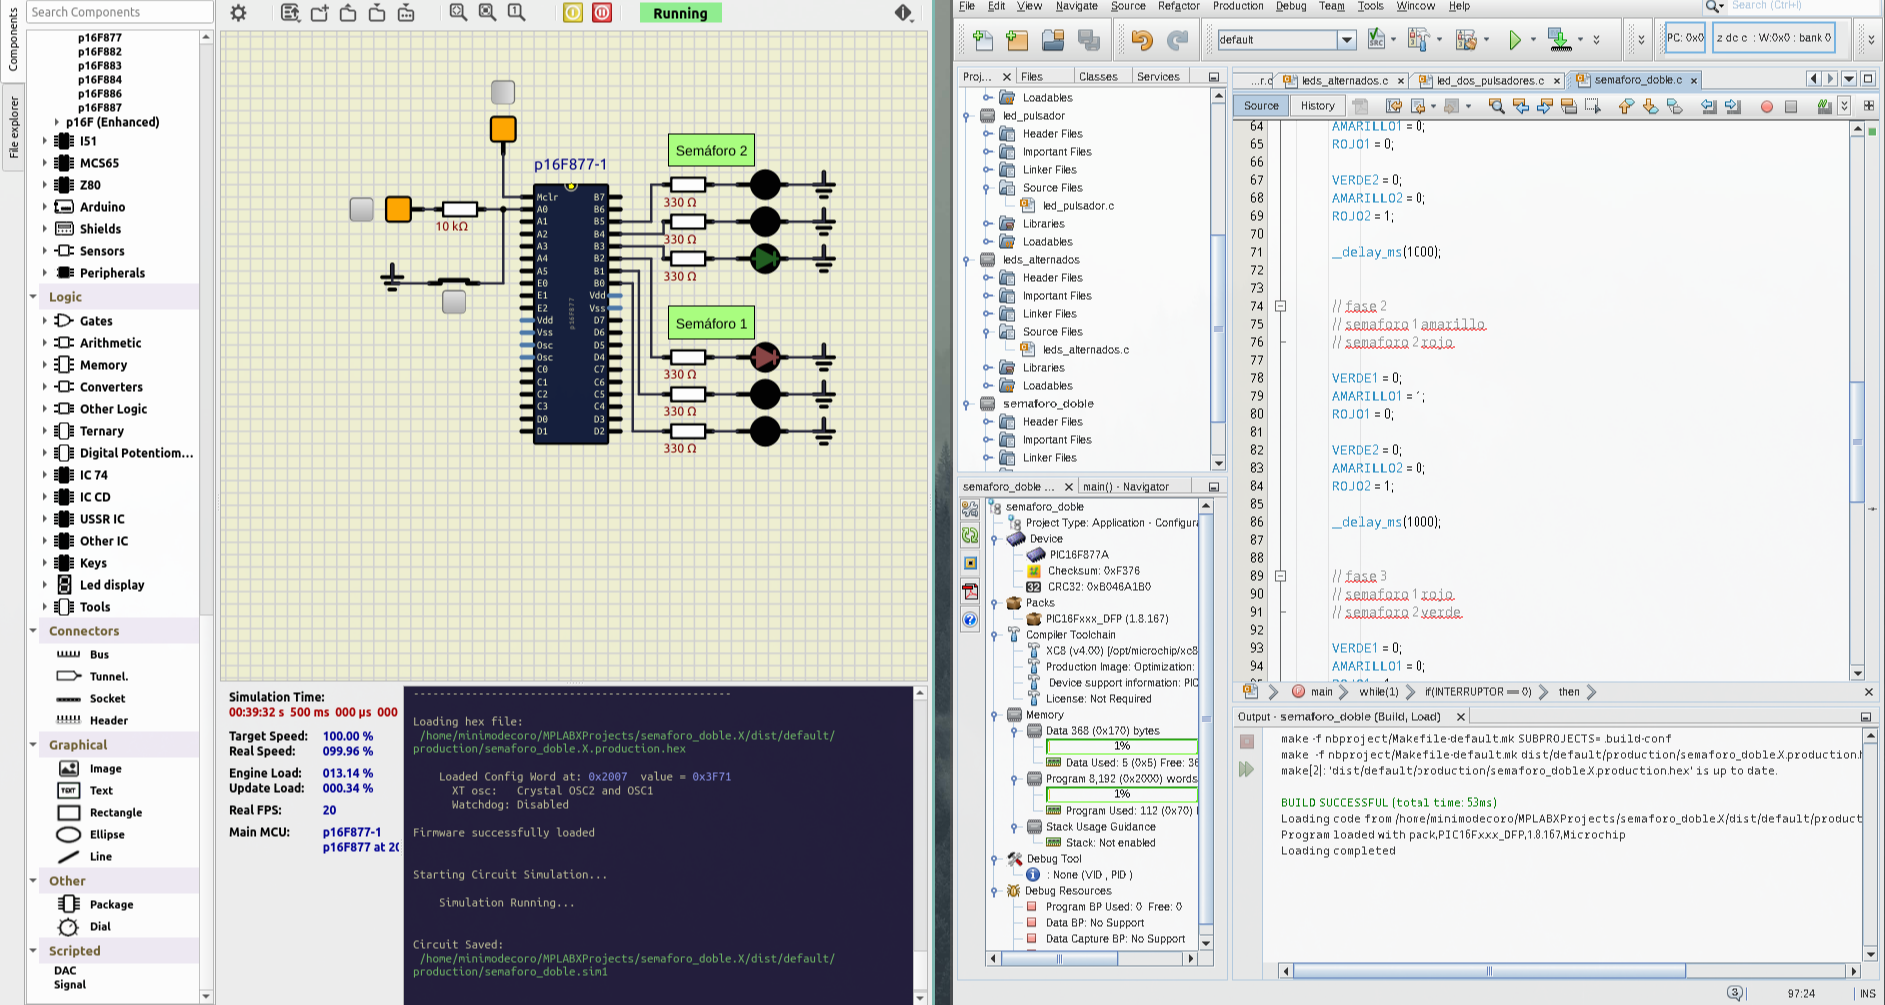
\includegraphics[
        width=0.9\textwidth,
        height=0.7\textheight,
        keepaspectratio
    ]{actividad5_fase3.png}

    \caption{Fase 3: semáforo 1 en rojo y semáforo 2 en verde.}
\end{figure}

\subsection{Fase 4}

Finalmente, en la cuarta fase el semáforo 1 permanece en rojo y el semáforo 2 cambia a amarillo.

\begin{figure}[H]
    \centering

    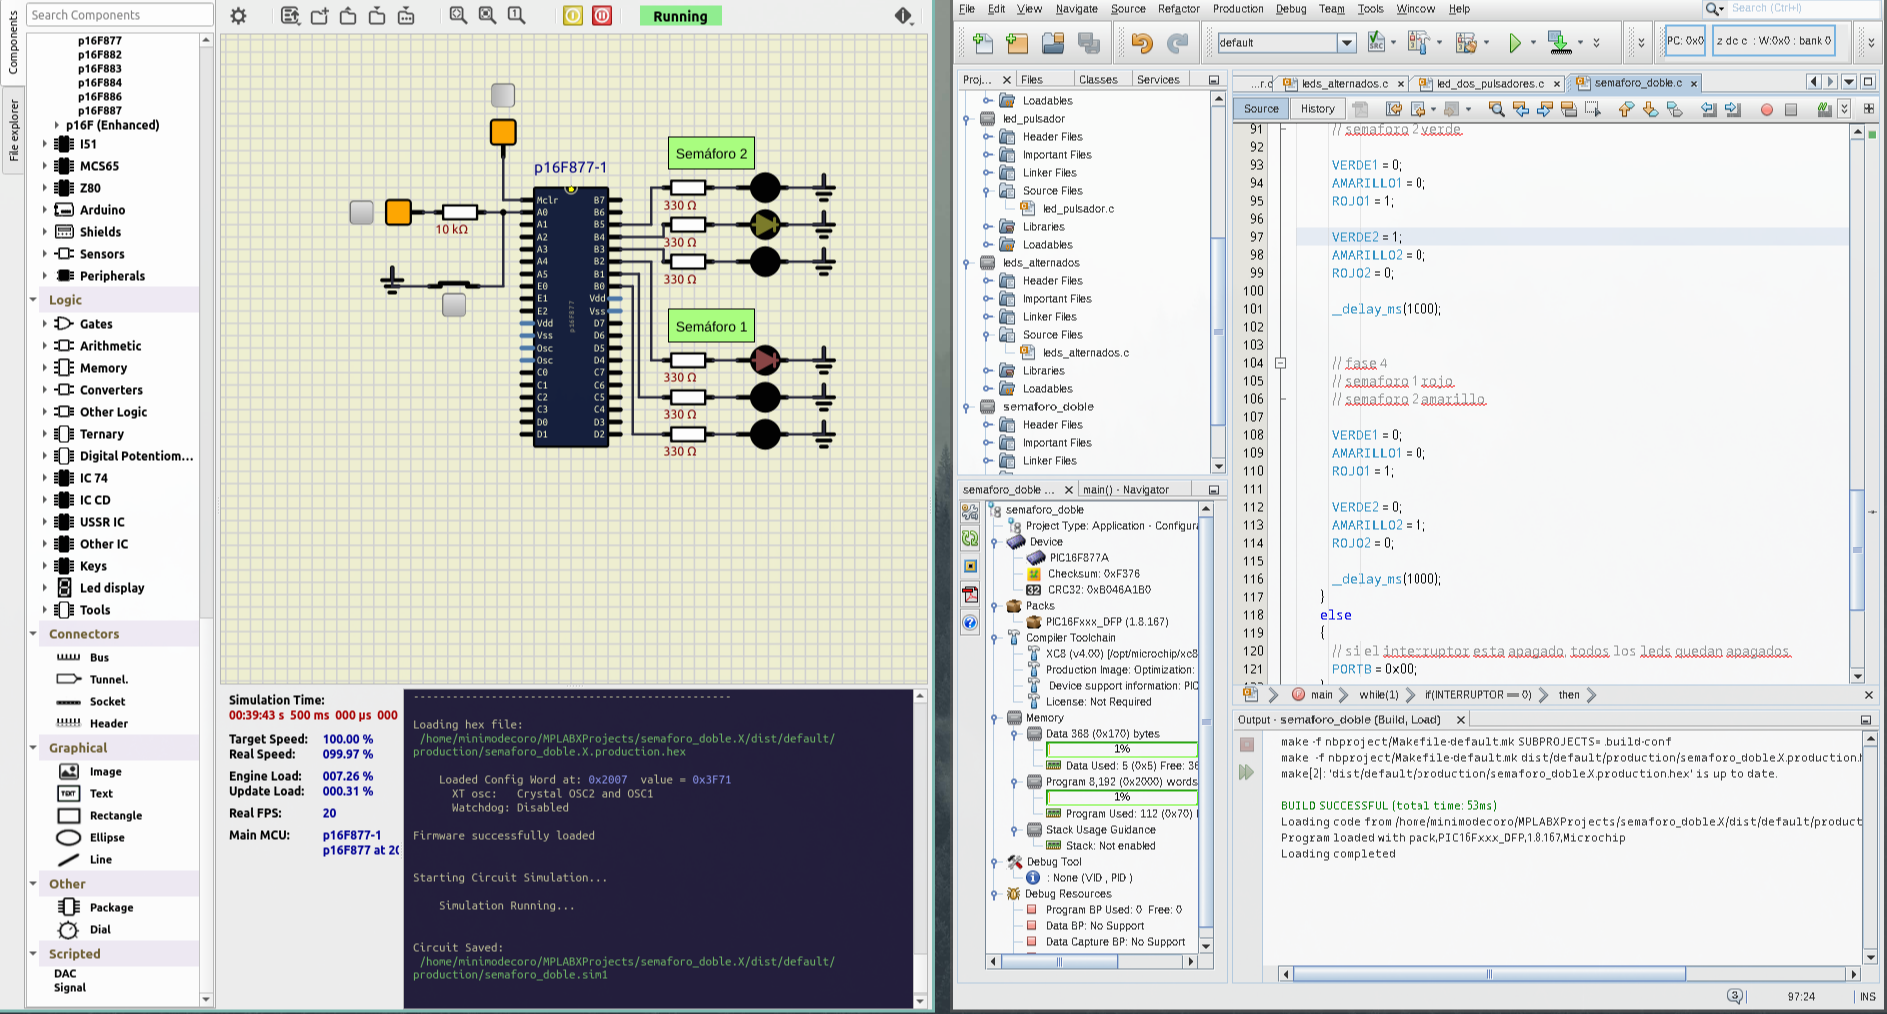
\includegraphics[
        width=0.9\textwidth,
        height=0.7\textheight,
        keepaspectratio
    ]{actividad5_fase4.png}

    \caption{Fase 4: semáforo 1 en rojo y semáforo 2 en amarillo.}
\end{figure}

\clearpage

% =========================================================
% DIFICULTADES Y APRENDIZAJES
% =========================================================

\section{Dificultades y aprendizajes durante el desarrollo}

Durante el desarrollo de las actividades también fueron apareciendo distintas dificultades que nos ayudaron a comprender de mejor manera cómo se relacionan el programa, la configuración del microcontrolador y el circuito simulado.

Una de las primeras confusiones estuvo relacionada con la configuración de los pines como entradas o salidas. Al comenzar las actividades era necesario entender qué significaban los registros TRIS y cómo un valor 0 configura un pin como salida, mientras que un valor 1 lo configura como entrada. Esto se volvió más claro al avanzar desde el primer ejercicio, donde solamente se controlaba un LED, hacia los ejercicios que incorporaban uno o más pulsadores.

Al comenzar a utilizar el puerto A también tuvimos que considerar que algunos de sus pines pueden funcionar como entradas analógicas. Por esta razón fue necesario utilizar la configuración de ADCON1 para poder trabajar con RA0 y RA1 como entradas digitales. Este fue un detalle que inicialmente no era tan evidente solamente observando el circuito, ya que también dependía de la configuración realizada desde el programa.

Otra dificultad importante fue comprender la lógica de los pulsadores utilizando resistencias pull-up. En un comienzo podía resultar confuso que un pulsador presionado correspondiera a un estado lógico 0 y que, al estar sin presionar, la entrada tuviera un estado lógico 1. Al probarlo directamente en las simulaciones pudimos relacionar de mejor manera el estado eléctrico de la entrada con las condiciones utilizadas en las estructuras \texttt{if} del código.

Durante las simulaciones también aparecieron problemas relacionados con la configuración del entorno. Fue necesario verificar que la frecuencia configurada en SimulIDE coincidiera con los 4 MHz definidos mediante \texttt{\_XTAL\_FREQ}, ya que esta frecuencia se utiliza para calcular correctamente los retardos del programa. También fue necesario mantener el pin MCLR en un nivel lógico alto para evitar que el microcontrolador permaneciera en estado de reset.

Otro aprendizaje fue distinguir entre compilar el proyecto y generar correctamente el archivo \texttt{.hex} utilizado por SimulIDE. Para las actividades se utilizó la compilación de producción de MPLAB X y posteriormente se cargó el archivo generado en el microcontrolador de la simulación. Esto permitió comprender un poco mejor el proceso que existe entre escribir el código en C y finalmente ejecutarlo en el PIC.

A medida que aumentó la cantidad de componentes también se volvió más importante mantener un orden entre los pines utilizados en el programa y las conexiones realizadas en el circuito. Por ejemplo, en las actividades con dos pulsadores y posteriormente en el semáforo fue necesario revisar que cada entrada y salida estuviera conectada al pin definido en el código, ya que una conexión realizada en un pin diferente podía provocar que el programa estuviera correcto pero que la simulación no respondiera como se esperaba.

Finalmente, la actividad de los dos semáforos nos permitió reunir gran parte de lo aprendido anteriormente. Al tener seis LED funcionando como salidas y un interruptor como entrada, fue necesario organizar tanto el circuito como el programa de una forma más clara. La división de la secuencia en cuatro fases permitió entender cómo una serie de instrucciones simples puede utilizarse para construir un comportamiento más completo.


% =========================================================
% CONCLUSION
% =========================================================

\section{Conclusión}

En este trabajo pudimos aplicar de forma práctica el manejo de entradas y salidas digitales del PIC16F877A, utilizando MPLAB X junto al compilador XC8 para programar y generar los archivos \texttt{.hex}, y SimulIDE para comprobar el funcionamiento de los circuitos.

Primero trabajamos con una salida simple haciendo parpadear un LED, después agregamos pulsadores como entradas y fuimos aumentando progresivamente la cantidad de entradas y salidas utilizadas, hasta llegar al control de dos semáforos.

A través de las actividades pudimos comprender mejor cómo funcionan los registros TRIS para definir si un pin se utiliza como entrada o salida, además del uso de PORT para controlar los estados de los pines. También trabajamos con la configuración de ADCON1 para poder utilizar los pines del puerto A como entradas digitales.

El uso de resistencias pull-up también permitió comprender la lógica utilizada por los pulsadores, donde la entrada permanece normalmente en estado lógico alto y cambia a estado lógico bajo al ser accionada.

Finalmente, la actividad del semáforo permitió integrar los conceptos anteriores en una secuencia de control más completa, utilizando seis salidas, una entrada y tiempos definidos para controlar los diferentes estados de ambos semáforos.

En general, el trabajo nos permitió relacionar de una forma más clara el código realizado en C con el comportamiento de las entradas y salidas del microcontrolador dentro de la simulación. Además, los errores y dificultades que fueron apareciendo durante las actividades fueron útiles para comprender que el funcionamiento de un sistema con microcontroladores no depende solamente del código, sino también de la configuración del PIC, de las conexiones realizadas y de que exista coherencia entre el programa y el circuito.

\end{document}